\documentclass[11pt,handout]{beamer}
%\documentclass[9pt]{beamer}
\usetheme[white]{Wisconsin}
%\title[short title]{long title}
\title[Oh hi]{Why Hello}
%\subtitle[short subtitle]{long subtitle}
\subtitle[Preliminary Examination]{Presentation of the Preliminary Report}
%\author[short name]{long name}
\author[A. Opotowsky]{Arrielle Opotowsky}
%\date[short date]{long date}
\date[29.01.2018]{29 January 2018}
%\institution[short name]{long name}
\institute[UW-Madison]{University of Wisconsin-Madison}

\usepackage{listings}
\usepackage{amsfonts}
\usepackage{amsmath}
\usepackage{xspace}
\usepackage{graphicx}
\usepackage{subfigure}
\usepackage{booktabs} % nice rules for tables
\usepackage{microtype} % if using PDF
\usepackage{bigints}
\newcommand{\units}[1] {\:\text{#1}}%
\setbeamertemplate{footline}[page number]
\setbeamertemplate{caption}[numbered]
\setbeamertemplate{bibliography item}[text]

%try to get rid of header on title page\dots
\makeatletter
    \newenvironment{withoutheadline}{
       \setbeamertemplate{headline}[default]
       \def\beamer@entrycode{\vspace*{-\headheight}}
    }{}
\makeatother

\begin{document}
%%%%%%%%%%%%%%%%%%%%%%%%%%%%%%%%%%%%%%%%%%%%%%%%%%%%%%%%%%%%%
%% From uw-beamer Here's a handy bit of code to place at 
%% the beginning of your presentation (after \begin{document}):
\newcommand*{\alphabet}{ABCDEFGHIJKLMNOPQRSTUVWXYZabcdefghijklmnopqrstuvwxyz}
\newlength{\highlightheight}
\newlength{\highlightdepth}
\newlength{\highlightmargin}
\setlength{\highlightmargin}{2pt}
\settoheight{\highlightheight}{\alphabet}
\settodepth{\highlightdepth}{\alphabet}
\addtolength{\highlightheight}{\highlightmargin}
\addtolength{\highlightdepth}{\highlightmargin}
\addtolength{\highlightheight}{\highlightdepth}
\newcommand*{\Highlight}{\rlap{\textcolor{HighlightBackground}{\rule[-\highlightdepth]{\linewidth}{\highlightheight}}}}
%%%%%%%%%%%%%%%%%%%%%%%%%%%%%%%%%%%%%%%%%%%%%%%%%%%%%%%%%%%%%
%%--------------------------------%%
\begin{withoutheadline}
\frame{
  \titlepage
  }
\end{withoutheadline}

%%--------------------------------%%
\AtBeginSection[]{
\begin{frame}
  \frametitle{Outline}
  \tableofcontents[currentsection]
\end{frame}
}

%\begin{frame}
%  \frametitle{X}
%  \begin{figure}[h!]
%    \centering
%    \includegraphics[width=0.9\textwidth]{.png}
%    \caption{x}
%    \label{fig:x}
%  \end{figure}
%\end{frame}

\section{Introduction}
\subsection{Motivation}
\begin{frame}
  \frametitle{Nuclear Security and Forensics}
  background here of what it is
\end{frame}

\begin{frame}
  \frametitle{Needs in Nuclear Forensics}
  US/DHS stuff plus NF-specific needs
\end{frame}


%\subsection{Methodology}
%
\begin{frame}
  \frametitle{Contribution of Computational Methods}
  \begin{figure}[h!]
    \centering
    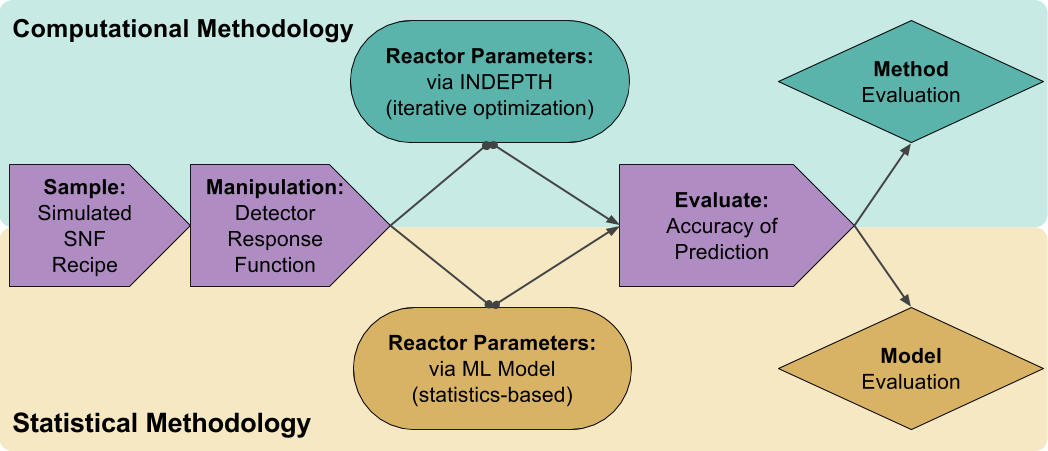
\includegraphics[width=0.9\textwidth]{CompStatForensicsWorkflow.png}
    \caption{Nuclear forensics research: physical, experimental, and computational}
  \end{figure}
\end{frame}

\begin{frame}
  \frametitle{Computational Methods}
  \begin{figure}[h!]
    \centering
    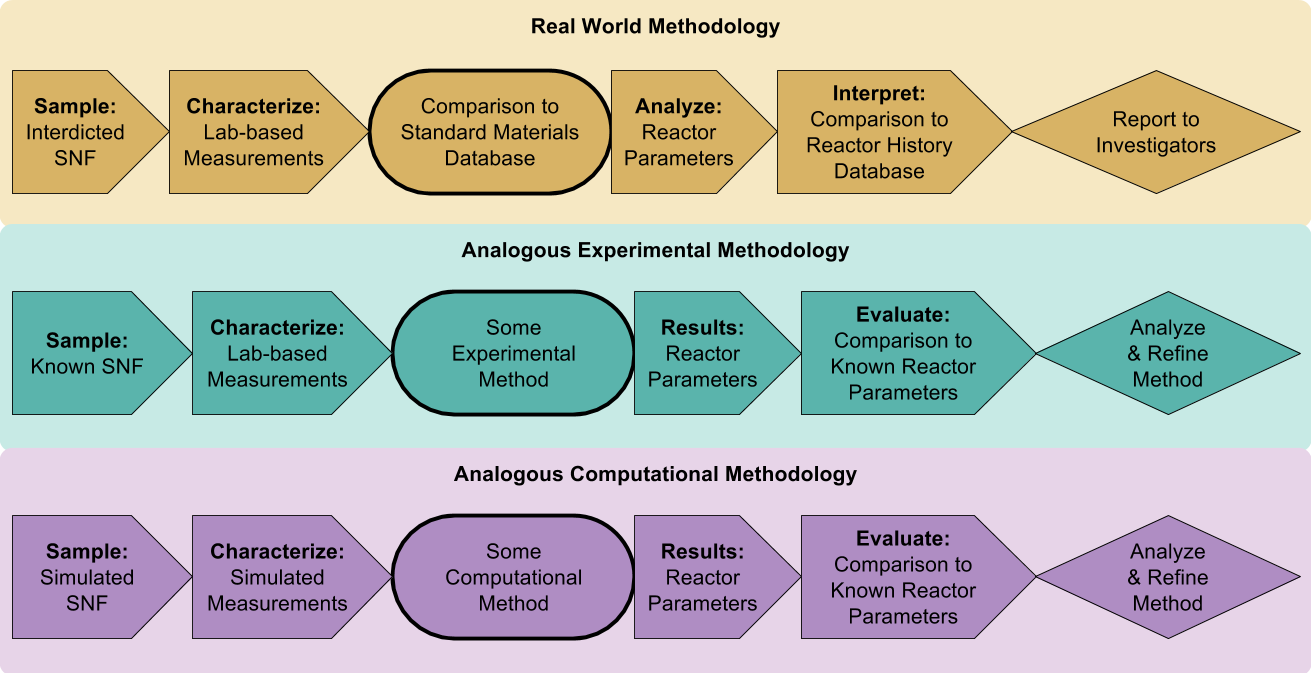
\includegraphics[width=0.9\textwidth]{ForensicsWorkflows.png}
    \caption{Comparison of computational approaches to nuclear forensics research}
  \end{figure}
\end{frame}

\begin{frame}
  \frametitle{Contribution of Statistical Methods}
  hi
\end{frame}

\begin{frame}
  \frametitle{Statistical Methods}
  hi
  %\begin{figure}[h!]
  %  \centering
  %  \includegraphics[width=0.9\textwidth]{xx.png}
  %  \caption{xx}
  %\end{figure}
\end{frame}

\begin{frame}
  \frametitle{Goal/Big Question}
  How does the ability to determine forensic-relevant spent nuclear fuel
  attributes using machine learning techniques degrade as less information is
  available?.
\end{frame}

%\subsection{Goals}
%\subsection{goals}

\section{Background}
%\subsection{Nuclear Forensics}
%The process of technical nuclear forensics includes the analysis and
interpretation of nuclear material to determine its history, whether that be
intercepted \gls{SNF}, \gls{UOC}, or the debris from an exploded nuclear
device. After the technical portion is complete, intelligence data can be used
to aid in material attribution; this is the overall goal of nuclear forensics. 

After a nuclear incident, the material or debris is sampled and evaluated
through many techniques that provide the following information: material
structure, chemical and elemental measurements, and radioisotope measurements.
These measurements or calculated ratios comprise the forensic signatures of the
sample in question. These signatures can be analyzed with specific domain
knowledge; for example, \gls{UOC} will have trace elements depending on where
it was mined from.  They can also be analyzed against a forensics database, in
the case of \gls{SNF}.

Measurement needs and techniques vary vastly depending on the material, as does
the type of signature. This study focuses on non-detonated materials,
specifically, \gls{SNF}. It is important to determine if some intercepted
material is from an undisclosed reactor or a commercial fuel cycle to attribute
it to an entity or state. This is typically done by obtaining chemical and
elemental signatures as well as isotopic ratios, and comparing these
measurements to those in an existing forensics database of reference \gls{SNF}. 

The signatures for \gls{SNF} correlate to several characteristics of quantities
that can, in a best case scenario, point to the exact reactor from which the
fuel was intercepted. The reactor parameters of interest are the reactor type,
fuel type and enrichment at beginning of irradiation, cooling time, burnup.
\todo{need citation, prob ORNL paper} \todo{more deets here? prob better later}

The current and future work of this study are designed based on two primary
needs to bolster the \gls{US} nuclear forensics capability: forensics databases
are imperfect, and our best measurement techniques are not always feasible in
an emergency scenario. It is proposed that using a machine-learned model may be
able to combat these issues, discussed in Section \todo{ref}. 

Forensics databases are kept by individual countries, and a given database will
have widely varying uncertainty depending where and on what instrument the
material was measured. Additionally, some fields have missing data. This
presents issues with matching and characterizing \gls{SNF} based on
interpolating between entries. \todo{more deets and cite}

A lofty goal for the forensics community would be to develop methods that
provide instantaneous information, reliable enough to guide an investigation
(e.g., within 24 hours). In the case of \gls{SNF}, it takes weeks in a lab to
measure isotopes via advanced gamma and mass spectroscopy equipment. Thus, fast
measurements to provide isotopic ratios to calculate the above-mentioned fuel
parameters of interest would provide this via some form of a handheld detector
that measures gamma spectra.  However, while this nondestructive analysis is
rapid, it is also difficult to evaluate because of the presence of overlapping
peaks. Thus, gamma spectra give less information at a higher uncertainty than
the near-perfect results of some destructive mass spectroscopy techniques, like
TIMS\todo{find MS technique and citation}.  Additionally, within gamma
spectroscopy techniques (e.g., field vs. lab detectors), uncertainties can vary
significantly because of the detector reponse, environment, storage,
electronics, etc. \todo{fix up and summary}


%\subsection{Statistical Models}
%%intro 
\begin{frame}
  \frametitle{Machine Learning}
  machine vs. statistical (domain knowledge->none)
  
  supervised and unsupervised
  
  clustering, dimensionality reduction

  classification, regression -- discrete and continuous variables
\end{frame}

%vocab
\begin{frame}
  \frametitle{Vocabulary}
  labels
  
  features
  
  generalizability
  
  prediction error

  objective error metric v prediction error metric
\end{frame}

%demo
\begin{frame}
  \frametitle{Supervised Regression}
  \begin{figure}[h!]
    \centering
    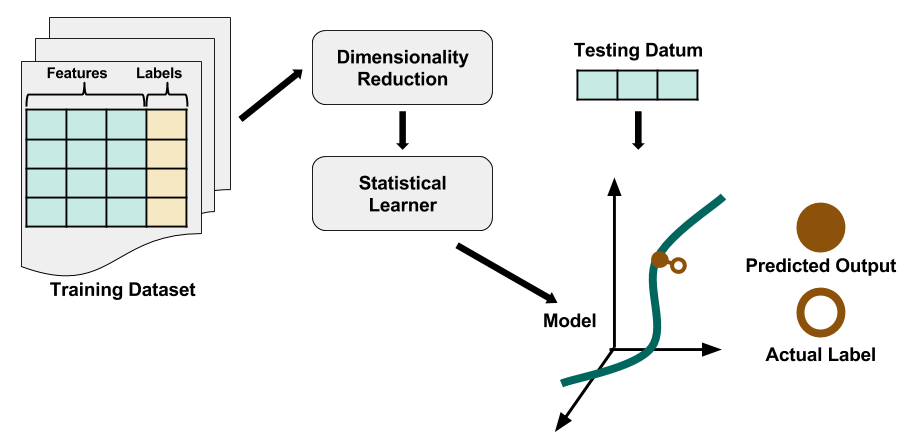
\includegraphics[width=0.9\textwidth]{./figures/SupervisedRegression.png}
    \caption{Schematic of a representative prediction workflow}
  \end{figure}
\end{frame}


%\subsection{Computational Tools}
%
\begin{frame}
  \frametitle{Computational Tools}
  \begin{itemize}
    \item Training Data : SNF recipes from SCALE/ORIGEN-ARP \cite{scale, origen}
    \item Information Reduction
    \begin{itemize}
      \item Gamma energies: ORIGEN
      \item Computational gamma spectra: GADRAS \cite{gadras}
    \end{itemize}
    \item Statistics Toolkit : scikit-learn (python) \cite{scikit}
  \end{itemize}
\end{frame}


%\subsection{Previous }
%%intro 
\begin{frame}
  \frametitle{Machine Learning}
  machine vs. statistical (domain knowledge->none)
  
  supervised and unsupervised
  
  clustering, dimensionality reduction

  classification, regression -- discrete and continuous variables
\end{frame}

%vocab
\begin{frame}
  \frametitle{Vocabulary}
  labels
  
  features
  
  generalizability
  
  prediction error

  objective error metric v prediction error metric
\end{frame}

%demo
\begin{frame}
  \frametitle{Supervised Regression}
  \begin{figure}[h!]
    \centering
    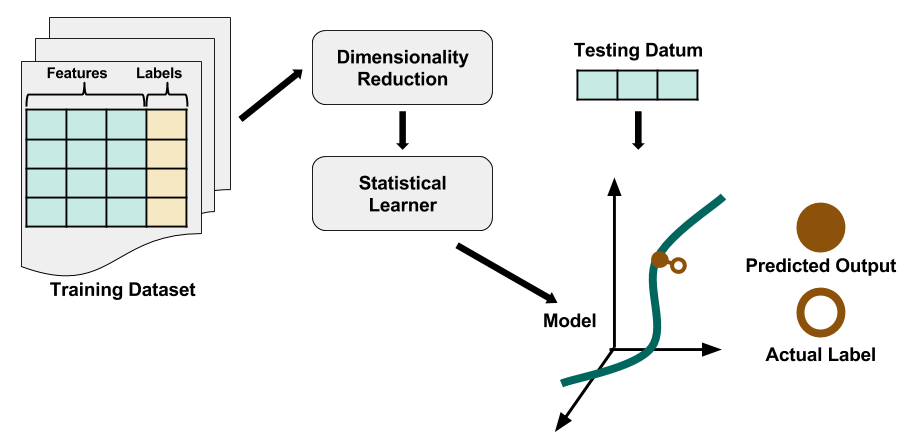
\includegraphics[width=0.9\textwidth]{./figures/SupervisedRegression.png}
    \caption{Schematic of a representative prediction workflow}
  \end{figure}
\end{frame}




\section{Demonstration}
%\input{demo}

\section{Research Proposal}
%\subsection{Experiment 1}
%
\begin{frame}
  \frametitle{Statistical Learning with Direct Isotopics}
  \textbf{Goals} : Understand limits of simplest scenario
  \begin{enumerate}
    \item Usefulness of statistical methods for reactor parameter prediction
    \item Best performing methods
  \end{enumerate}

  \textbf{Variables}
  \begin{enumerate}
    \item the complexity of the ML algorithm used, 
    \item feature reduction, and 
    \item different subsets of the decision space.
  \end{enumerate}
\end{frame}

\begin{frame}
  \frametitle{Statistical Learning with Direct Isotopics}
  \textbf{Qualitative Hypotheses}
  \begin{itemize}
    \item Complex algorithm will provide best behavior
    \item Manual preprocessing (feature reduction): speed, accuracy
    \item Reduction of decision space should help: PWR vs. BWR?
  \end{itemize}

  \textbf{Risk Mitigation}
  \begin{itemize}
    \item New algorithms: tree-based, neural nets, Bayesian MLE
    \item Statistical preprocessing: PCA, ICA
    \item New materials: Pu, UOC, Post-detonation (urban canyon \cite{refmaterial})
  \end{itemize}
\end{frame}


%\subsection{Experiment 2}
%
\begin{frame}
  \frametitle{Statistical Learning with Gamma Spectra}
  \textbf{Goals} : Understand limits of real-world scenario
  \begin{enumerate}
    \item Level of reduction in reactor parameter prediction
    \item Best performing methods
  \end{enumerate}

  \textbf{Variables}
  \begin{enumerate}
    \item the complexity of the ML algorithm used, 
    \item feature reduction (implicit), and 
    \item quality of training and/or testing data set.
  \end{enumerate}
\end{frame}

\begin{frame}
  \frametitle{Statistical Learning with Gamma Spectra}
  \textbf{Qualitative Hypotheses}
  \begin{itemize}
    \item Complex algorithm will provide best behavior
    \item Indirect isotopics $=$ implicit feature reduction: less accurate
    \item Higher quality gamma spectra will yield better results
  \end{itemize}

  \textbf{Risk Mitigation}
  \begin{itemize}
    \item New algorithms: tree-based, neural nets, Bayesian MLE
    \item Further manual or statistical preprocessing
    \item Add isotope identification step
  \end{itemize}
\end{frame}


%\subsection{Experiment 3}
%
\begin{frame}
  \frametitle{Viability of Statistical Learning on Reprocessed Fuel}
  Purpose

  Variables
\end{frame}

\begin{frame}
  \frametitle{Viability of Statistical Learning on Reprocessed Fuel}
  Hypotheses

  Risks
\end{frame}



\section{Conclusion}
%\subsection{Summary}
%\begin{frame}
  \frametitle{Summary}
  \textbf{Pre-detonation nuclear forensics analysis on SNF}
  \small
  \begin{itemize}
    \item Demonstrated:
    \begin{itemize}
      \item Simulation of training data set
      \item Information reduction of training set
      \item Burnup prediction using three statisitcal models: ridge, \textit{k}-nearest neighbor, and support vector regression
      \item ML model optimization via diagnostic curves
      \item Plan for ML model comparison
    \end{itemize}
    \item Simplifications:
    \begin{itemize}
      \item Only predicted burnup (missing rxtr type, enrichment, cooling time)
      \item Borrowed training set
      \item No statistical feature reduction
      \item No physically based information reduction
    \end{itemize}
    \item Three experiments:
    \begin{itemize}
      \item Nuclide concentrations
      \item Gamma energies/spectra
      \item Reprocessed SNF
    \end{itemize}
  \end{itemize}
\end{frame}

%\subsection{Future Work}
%\subsection{Next Steps}

This is how I will expand upon the experiments given the time.  So many
options.

Diff algs ()
Diff sims (SFCOMPO space represented bc this offers better real-world testing for more technologies)


The next step is to provide a larger, more diverse training set to the
algorithms so they could predict better when faced with new instances.  Dayman
training/test set -> sfcompo-like sims and testing set

To obtain reliable models, one must both choose or create a training set
carefully and study the impact of various algorithm parameters on the error.
Many algorithms are developed on an assumption that the training set will be \gls{i.i.d.}.
This is important so that the
model does not overvalue or overfit a certain area in the training space. 

\subsection{Long-term Plans}

dddd


%%--------------------------------%%
%%--------------------------------%%

\begin{frame}[allowframebreaks]
  \frametitle{References}
  \bibliographystyle{plain}
  {\footnotesize \bibliography{prelim} }
\end{frame}

%%--------------------------------%%

\end{document}


